\documentclass[a4paper,12pt]{book}
\usepackage{graphicx}
\usepackage[export]{adjustbox}
\usepackage{subcaption}
\graphicspath{{Pics/}}
\usepackage{charter}
\usepackage{fancyhdr}
\usepackage{enumerate}
\usepackage{enumitem}
\usepackage{siunitx}
\usepackage{amssymb}
\usepackage{longtable}
\usepackage{multicol}
\usepackage{multirow}
\usepackage{hhline}
\usepackage{parskip}
\setlength{\parskip}{6pt}
\usepackage{ragged2e}
\usepackage{geometry} %margin
\geometry{left=2.1cm,right=2.1cm,top=3cm,bottom=3cm}
\usepackage{setspace}
\SetSinglespace{1.2}
\singlespacing
\renewcommand{\ttfamily}{\fontfamily{pcr}\selectfont}
%\renewcommand{\familydefault}{\rmdefault}

\usepackage[,table]{xcolor}
\definecolor{LightBlue}{cmyk}{0.16,0.03,0.04,0}
\definecolor{Title}{cmyk}{0.8,0.1,0,0.3}
\setlength{\arrayrulewidth}{0.3mm}
\setlength{\tabcolsep}{2pt}
\setlength{\headheight}{15pt}
\renewcommand{\arraystretch}{1}
\usepackage{tikz}
\usepackage{nicematrix}
\newcommand*\circled[1]{\tikz[baseline=(char.base)]{\node[shape=circle,draw,inner sep=1pt] (char) {#1};}}

\newcolumntype{s}{>{\columncolor{Title}\RaggedLeft} m{3.5em}} % columntype for chapter title
\newcolumntype{d}{>{\columncolor{LightBlue}\RaggedRight} m{\textwidth}} % columntype for code bloc
\newcolumntype{a}{>{\columncolor{LightBlue}\RaggedRight} m{0.96\textwidth}} % columntype for secondary code bloc

\usepackage{titlesec}
\usepackage[hidelinks]{hyperref}
\urlstyle{same}

\captionsetup[figure]{labelsep=period,font={bf}}
\captionsetup[table]{font={bf},labelsep=period}

\newcommand{\titlename}{}

\newcommand{\chaptertitle}[2]{ %reset chapter format
\vspace{-120pt}
\gdef\titlename{#1}
{
\SetSinglespace{1.1}
\singlespacing
\Huge\bfseries
\setlength{\tabcolsep}{8pt}
\renewcommand{\arraystretch}{1.5}
\begin{tabular}{s >{\RaggedRight}m{14.5em}}
\textcolor{white}{Chapter\newline\thechapter}&\textcolor{Title}{#2}
\end{tabular}
}
}

\newcommand{\partpic}[1]{%insert picture
    \tikz[remember picture,overlay] \node at (current page.center){\includegraphics[width=\paperwidth]{#1}};
}

\titleformat{\part} %reset part %format
{\huge\bfseries} % format
{} % label
{0em} % sep
{\Centering} % before-code

\titleformat{\chapter} %reset chapter %format
{\huge\bfseries} % format
{} % label
{0em} % sep
{\Centering} % before-code
\titlespacing{\chapter}{0pt}{0pt}{0pt}

\titleformat{\section} %reset section %format
{\Large\bfseries} % format
{\textcolor{Title}{\thesection}} % label
{0.5em} % sep
{\color{Title}} % before-code
\titlespacing{\section}{0pt}{12pt}{6pt}

\titleformat{\subsection} %reset subsection %format
{\large\bfseries} % format
{\textcolor{Title}{\thesubsection}} % label
{0.5em} % sep
{\color{Title}} % before-code
\titlespacing{\subsection}{0pt}{8pt}{6pt}

\newenvironment{term}[1]{
    \textbf{#1}

    \leftskip 1em
    \parskip 0pt
}

\newenvironment{secterm}[1]{
    \textbf{#1}

    \leftskip 2em
    \parskip 0pt
}

\newenvironment{codebloc}{ %define code bloc style
    \ttfamily\footnotesize
    \renewcommand{\arraystretch}{1}
}

\newcommand{\note}[2][NOTE]{ %Note/Tips
\vspace{6pt}
\begin{tabular}{b{\textwidth}}
\hline
\fontfamily{phv}\selectfont \textbf{#1}\\
\leftskip 1em #2\\
\hline
\end{tabular}
}

\newcommand{\secnote}[2][NOTE]{ %Note/Tips
\vspace{6pt}
\begin{tabular}{b{0.93\textwidth}}
\hline
\fontfamily{phv}\selectfont \textbf{#1}\\
\leftskip 1em #2\\
\hline
\end{tabular}
}

\title{ESP32-C3 Wireless Adventure\par \Large A comprehensive guide to IoT}
\author{Espressif Systems}
\date{\today}

\pagestyle{fancy} % reset head&foot
\fancyhead{} % clear all header fields
\renewcommand\headrulewidth{0pt}
\fancyfoot{} % clear all footer fields
\setcounter{chapter}{14}

\begin{document}

\fancyfoot[LE]{\fontfamily{cmss}\selectfont{\textbf{\thepage} \ \textit{ESP32-C3 Wireless Adventure: A comprehensive guide to IoT}}}
\fancyfoot[RO]{\fontfamily{cmss}\selectfont{\textit{Chapter \thechapter. \titlename} \ \textbf{\thepage}}}

\chapter[ESP Insights: Remote Monitoring Platform]{\chaptertitle{ESP Insights: Remote Monitoring Platform}{ESP Insights:\newline Remote Monitoring Platform}}

\vspace{36pt}
The previous chapters introduced the ESP RainMaker IoT cloud platform, a device-to-cloud solution provided by Espressif. Using the components of the ESP RainMaker IoT cloud platform, users can easily connect to ESP RainMaker, realizing remote control of devices. With the help of the ESP RainMaker IoT cloud platform, users can develop the ESP32-C3 smart LED products with ease. But we all know that from project approval to mass production, a product needs to go through main processes including functional evaluation, implementation, and verification.

Based on the introduction about the functions of smart LED products and how these functions are realized from the previous chapters, you may wonder after realizing the functions of the smart LED, how to carry out systematic functional verification and on-hook verification.

After developing the function code of a project, functional verification is required. At this time, you can set the log level to Debug mode, and monitor the log on the serial port to get the debugging done. This is a necessary verification before releasing the software. Upon completing the basic functional verification, functions such as log output and command line debugging should often be disabled. Then, it’s time to release the Release version. Thereafter, even if the software behaves abnormally during the Quality Assurance (QA) test or during usage, it will be difficult for developers to quickly locate and fix the issues by obtaining device logs. Sometimes, developers may even need to disassemble the device for the logs to analyze the cause of the abnormality. To solve this problem, Espressif Systems has developed ESP Insights, which supports developers to check the running status and logs of firmware remotely, so as to detect and solve firmware problems in time, speeding up the software development process.

\section{Introduction to ESP Insights}
ESP Insights (project link: \url{https://github.com/espressif/esp-insights}) is a remote monitoring platform that allows users to monitor the health of the device remotely, including warning and error logs, metrics for device operating parameters, device coredump information, and custom data and events.

In this chapter, we will introduce the functions and applications of ESP Insights based on the \verb|esp-insights| project. The commit ID is \verb|afd70855eb4f456e7ef7dc233bf082ec7892|\\ \verb|d9df|.

ESP Insights includes a firmware agent, the Insights agent, that captures vital pieces of diagnostics information from the device during runtime and uploads them to the ESP Insights cloud. The cloud then processes this data for visualization. Developers can log in to a web-based dashboard to look at the health and issues reported by their devices in the field. Currently, we only support processing diagnostics information and reports on the ESP RainMaker IoT cloud platform. Support for other cloud platforms will be available in later releases. Figure 15.1 presents the ESP RainMaker IoT cloud platform overview report. Figure 15.2 presents the ESP RainMaker IoT cloud platform metrics report. Figure 15.3 presents the ESP RainMaker IoT cloud platform variables report.

\begin{figure}[!h]
    \centering
    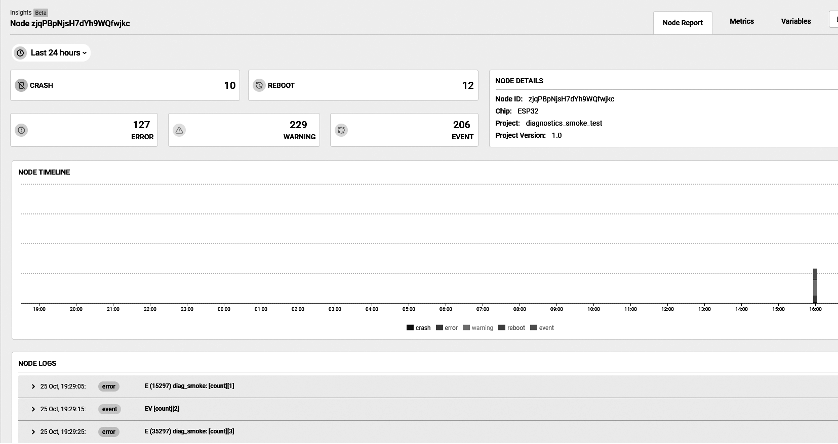
\includegraphics[width=0.85\textwidth]{D15Z/15-1}
    \caption{Overview report by ESP RainMaker}
\end{figure}

\begin{figure}[!h]
    \centering
    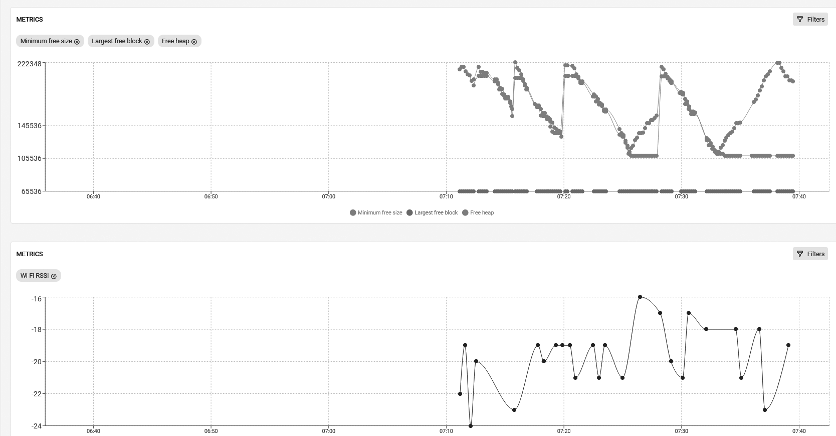
\includegraphics[width=0.9\textwidth]{D15Z/15-2}
    \caption{Metrics report by ESP RainMaker}
\end{figure}

\begin{figure}[!h]
    \centering
    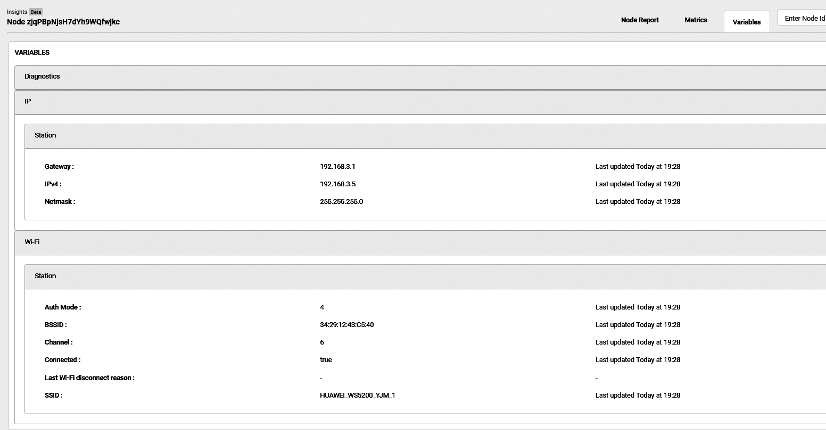
\includegraphics[width=0.9\textwidth]{D15Z/15-3}
    \caption{Variable report by ESP RainMaker}
\end{figure}

Currently, developers can monitor the following information on the web-based dashboard:

\begin{term}{Error logs}
     Outputs by the serial port when the log printing function \verb|ESP_LOGE()| is called by components or user applications.
\end{term}

\begin{term}{Warning logs}
     Outputs by the serial port when the log printing function \verb|ESP_LOGW()| is called by components or user applications.
\end{term}
     
\begin{term}{Custom events}
     Outputs by the serial port when \verb|ESP_DIAG_EVENT()| is called by user applications. Custom events can be used for user-defined data.
\end{term}

\begin{term}{Reset reason}
     Reasons why the device is reset, e.g., powered on, software reset, brownout, etc.
\end{term}

\begin{term}{Coredump summary}
     Register contents and stack backtrace of the offending thread in case of a crash.
\end{term}
     
\begin{term}{Metrics}
     Time-varying data, e.g., the free heap size, the Wi-Fi signal strength plotted over time, etc.
\end{term}
     
\begin{term}{Variables}
     Variable values, e.g., the device's IP address, gateway address, Wi-Fi connection information, etc.
\end{term}

\textbf{1. Features of ESP Insights}

\begin{enumerate}[label=(\arabic*)]
    \item Check device properties (e.g., name, ID, firmware version, etc.) and device status (e.g., memory usage, maximum free block, free heap value, Wi-Fi signal strength, etc.).
    \item Check logs generated during device firmware operation, such as error and warning logs, crash backtrace information, reboots, and other custom events.
    \item Check the current data reported by the device and generate data sheets according to time.
    \item Support customised metrics and variables based on users' needs.
\end{enumerate}

\textbf{2. Advantages of ESP Insights}

\begin{enumerate}[label=(\arabic*)]
    \item Accelerate the development and release of software products.
    
    Beta tests are normally required before releasing any software products officially. During the beta testing, users will provide feedback regarding the performance, stability, reliability, and other problems of the product in real usage scenarios, which will then be handled and fixed by developers. This process often costs developers a large amount of time and effort in locating problems and analysing the causes. With ESP Insights, developers can check the device operation status remotely and obtain the details of abnormal events in a timely manner, saving the time on handling problems greatly and accelerating the software development and release process. ESP Insights also saves the records of abnormal events occured before the device firmware crashes. After the device is rebooted, it uploads the data to the cloud, thus avoiding losing abnormal information.

    \item Handle various firmware problems in a timely manner. For example:

    \begin{enumerate}[label=\alph*.]
        \item Developers can use ESP Insights to check device status (such as available memory space, maximum free block, Wi-Fi signal strength, etc.), analyse the peak value of each metric of the device, and introduce optimisation in future firmware versions.
        \item The logs of ESP Insights record the details of all abnormal events, so that developers can handle the abnormality in time before it is detected by the user, preventing any impact of device abnormality on the actual use of the device.
    \end{enumerate}

    \item Data transmission: lightweight, simple, safe, and reliable.
    
    ESP Insights is capable of transmitting diagnostics data using the HTTPS protocol and the MQTT protocol. When working with the ESP RainMaker IoT cloud platform, ESP Insights supports sharing the diagnostics data transmitted over an encrypted channel via the MQTT protocol with the RainMaker IoT Cloud Platform, greatly reducing the memory usage of the device while ensuring the information security. If you are not using the ESP RainMaker IoT cloud platform, you can use the HTTPS protocol alone to transfer the diagnostics data. However, compared with the ESP RainMaker IoT cloud platform, using the HTTPS protocol alone requires adding a TLS link, which will lead to increased memory usage. The data transmitted between the device and the cloud platform is optimised by the CBOR encoding, which significantly saves data transmission bandwidth. In the future, ESP Insights will also integrate device data with the command and control data from the cloud, and pack them into the same MQTT message, further reducing costs with fewer MQTT messages.
\end{enumerate}

\section{Getting Started with ESP Insights}
Following the features and advantages of ESP Insights, in this section, we will explain how to get started with ESP Insights based on the \verb|esp-insights| project and how to check the information reported by the device on the remote dashboard.

\subsection{Getting Started with ESP Insights in the esp-insights Project}
To get started with ESP Insights in the \verb|esp-insights| project, please follow the steps below:

\textbf{1. Clone the latest esp-RainMaker}

Based on the previous introduction to the ESP RainMaker IoT cloud platform, pull the project code of \verb|esp-RainMaker|, and \verb|esp-insights| will be under the project directory \verb|esp-RainMaker/components| as a submodule.

\begin{codebloc}
\begin{tabular}{d}
\$ \textbf{git clone --recursive https://github.com/espressif/esp-RainMaker.git}
\end{tabular}
\end{codebloc}

\textbf{2. Modify CMakeLists.txt of esp-RainMaker}

Add \verb|esp-insight| as a component to the \verb|esp-RainMaker| project, ensuring that the functions of \verb|esp-insight| can be called under the \verb|esp-RainMaker| project. In the current directory of building project, modify the following command in \verb|CMakeLists.txt|:

\begin{codebloc}
\begin{tabular}{d}
\verb|1.  set(EXTRA_COMPONENT_DIRS ${RMAKER_PATH}/components ${RMAKER_PATH}/examples/|\\
\verb|common)|
\end{tabular}
\end{codebloc}

to:

\begin{codebloc}
\begin{tabular}{d}
\verb|1.  set(EXTRA_COMPONENT_DIRS ${RMAKER_PATH}/components ${RMAKER_PATH}/examples/|\\
\verb|common ${RMAKER_PATH}/components/esp-insights/components)|
\end{tabular}
\end{codebloc}

\textbf{3. Implement the features of ESP Insights}

The code for ESP Insights is already wrapped by the \verb|examples/common/app_insights| component. Users only need to include \verb|app_insights.h| in their code and call \verb|app_|\\ \verb|insights_enable()| before calling \verb|esp_rmaker_start()|. However, this component is controlled by the macro \verb|CONFIG_ESP_INSIGHTS_ENABLED|, which is disabled by default. Users can enable this feature in default configuration or the image configuration interface (use the \verb|idf.py| tool to open the menu \verb|menuconfig| → \verb|Component config| → \verb|ESP Insights| → \verb|Enable ESP Insights|).

\textbf{4. Build and flash}

Run the following command to build and flash:

\begin{codebloc}
\begin{tabular}{d}
\$ \textbf{idf.py build flash monitor}
\end{tabular}
\end{codebloc}

When the build completes, the following log will be printed as an \verb|led_light-v1.0.zip| will be generated in the \verb|build| directory for future use.

\begin{codebloc}
\begin{tabular}{d}
\vspace{2pt}
\begin{verbatim}
======= Generating insights firmware package build/led_light-v1.0.zip =========
led_light-v1.0
led_light-v1.0/led_light.bin
led_light-v1.0/sdkconfig
led_light-v1.0/partition_table
led_light-v1.0/partition_table/partition-table.bin
led_light-v1.0/bootloader
led_light-v1.0/bootloader/bootloader.bin
led_light-v1.0/partitions.csv
led_light-v1.0/project_build_config.json
led_light-v1.0/led_light.map
led_light-v1.0/led_light.elf
\end{verbatim}
\verb|led_light-v1.0/project_description.json|
\end{tabular}
\end{codebloc}

\textbf{5. Claiming for the ESP RainMaker IoT cloud platform}

As developers need the admin access for the ESP Insights cloud, claiming is thus required. For specific claiming details, please refer to Chapter 3.

\textbf{6. Log in to the Dashboard of ESP RainMaker}

Once the firmware and claiming operations are all completed, the device is ready to connect to ESP RainMaker. Now, users can log in to the ESP RainMaker interface (\url{https://dashboard.RainMaker.espressif.com/}), and click the node corresponding to the device to enter its Dashboard.

\textbf{7. Upload the generated zip file}

To better understand the diagnostics information, users also need to upload the previously generated zip file \verb|led_light-v1.0.zip| to \verb|Firmware Images| on the left navigation bar of the ESP RainMaker interface, as the zip file contains binary files, elf files, mapping files, and other useful information for analysis.

Even without changes in code, commands such as \verb|idf.py build| and \verb|idf.py flash| will conduct rebuilds to generate new firmware. Thus, it is important to ensure that the firmware running on the device corresponds to the zip file package uploaded to the ESP RainMaker platform. Otherwise, ESP RainMaker may report errors when processing and analysing the information reported by the device.

\subsection{Running Example in the esp-insights Project}

\textbf{1. Clone ESP Insights}

Clone the project code for ESP Insights using the command below:

\begin{codebloc}
\begin{tabular}{d}
\$ \textbf{git clone --recursive https://github.com/espressif/esp-insights.git}
\end{tabular}
\end{codebloc}

\textbf{2. Configure ESP-IDF}

ESP Insights currently supports the master branch and v4.3.x, v4.2.x, and v4.1.x release branches.

To get the support for v4.3.2, you need to run the following command for a patch:

\begin{codebloc}
\begin{tabular}{d}
\$ \textbf{cd \$IDF\_PATH}\\
\$ \textbf{git apply -v <path/to/esp-insights>/idf-patches/Diagnostics-support-in-esp-}\\
\textbf{idf-tag-v4.3.2.patch}
\end{tabular}
\end{codebloc}

To get the support for v4.2.2 and v4.0.0, the following command is needed for a patch:

\begin{codebloc}
\begin{tabular}{d}
\$ \textbf{cd \$IDF\_PATH}\\
\$ \textbf{git apply -v <path/to/esp-insights>/idf-patches/Diagnostics-support-in-esp-}\\
\textbf{idf-tag-v4.1.1-and-tag-v4.22.patch}
\end{tabular}
\end{codebloc}

Users can choose the HTTPS protocol or the MQTT protocol to transmit diagnostics data according to the needs. For specific configurations, please refer to the following command:

\begin{codebloc}
\begin{tabular}{d}
\$ \textbf{idf.py menuconfig}
\end{tabular}
\end{codebloc}

Navigate to \verb|Component config|→\verb|ESP Insights|→\verb|Insights default transports|.

If the HTTPS protocol is selected to transmit diagnostics data, users need to log in to \url{https://dashboard.insights.espressif.com/home/insights} to check the diagnostics log for the device.

\textbf{3. Build and flash}

Refer to step 4-7 in Section 15.2.1.

\subsection{Reporting Coredump Information}
In case of a firmware crash, the Insights agent captures the coredump information into the flash memory and reports it to the ESP Insights cloud in the subsequent boot-up. This allows you to look at all the crash logs that the devices may be generating in the field.

The entire stack backtrace leading up to the crash is also captured and reported. To optimise the device-cloud communication, the firmware only sends a summary of the coredump. The summary contains the most useful contents of the coredump like program counter, exception cause, exception address, general purpose registers, and the backtrace. Figure 15.4 shows a piece of coredump information.

\begin{figure}[!h]
    \centering
    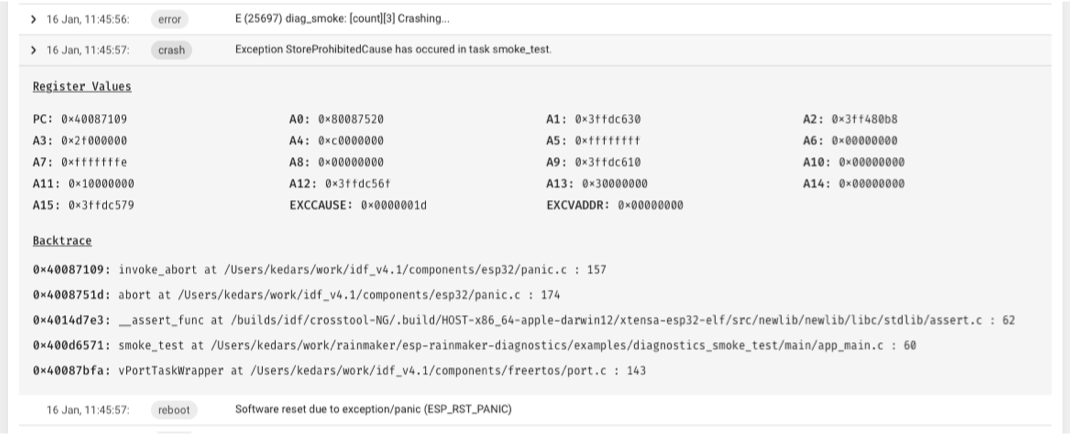
\includegraphics[width=0.9\textwidth]{D15Z/15-4}
    \caption{Coredump information}
\end{figure}

This feature requires the following configurations, which should be added to the project's default configuration file \verb|sdkconfig.defaults|.

\begin{codebloc}
\begin{tabular}{d}
\vspace{2pt}
\begin{verbatim}
1.  CONFIG_ESP32_ENABLE_COREDUMP=y
2.  CONFIG_ESP32_ENABLE_COREDUMP_TO_FLASH=y
3.  CONFIG_ESP32_COREDUMP_DATA_FORMAT_ELF=y
4.  CONFIG_ESP32_COREDUMP_CHECKSUM_CRC32=y
\end{verbatim}
\verb|5.  CONFIG_ESP32_CORE_DUMP_MAX_TASKS_NUM=64|
\end{tabular}
\end{codebloc}

To store the coredump into flash, an additional coredump partition is required. Add the following line to the \verb|partitions.csv| of the project.

\begin{codebloc}
\begin{tabular}{d}
\verb|1.  coredump, data, coredump, , 64K|
\end{tabular}
\end{codebloc}

\subsection{Customising Logs of Interest}
\verb|esp_log| is the default logging component in ESP-IDF. Typically, \verb|ESP_LOGE| and \verb|ESP_LOGW| are used to log errors and warnings in the firmware. All logs recorded using the \verb|esp_log| component are tracked by the Insights agent and reported to the ESP Insights cloud. This allows developers to view these errors through the ESP Insights Dashboard, providing detailed information about what may be going on.

Developers can configure the log level by calling \verb|esp_diag_log_hook_enable()| and \verb|esp_diag_log_hook_disable()|.

\begin{codebloc}
\begin{tabular}{d}
\vspace{2pt}
\begin{verbatim}
1.  /*enable tracking error logs*/
2.  esp_diag_log_hook_enable(ESP_DIAG_LOG_TYPE_ERROR);
3.
4.  /*enable tracking all log levels*/
5.  esp_diag_log_hook_enable(ESP_DIAG_LOG_TYPE_ERROR|ESP_DIAG_LOG_TYPE_WARNING|
6.  ESP_DIAG_LOG_TYPE_EVENT);
7.
8.  /*disable tracking custom events*/
\end{verbatim}
\verb|9.  esp_diag_log_hook_disable(ESP_DIAG_LOG_TYPE_EVENT);|
\end{tabular}
\end{codebloc}

Normally, some error or warning logs are printed before the device crashes, which are hard to be reported to the cloud. ESP Insights agent provides a way to keep the logs and report them to the ESP Insights cloud after boot-up. ESP32-C3 is equipped with RTC memory. The Insights agent uses this memory to store the critical errors that occurred in the system. On any boot-up, the Insights agent will check for any unreported errors from the previous boot-up through this RTC memory and report that to the ESP Insights cloud.

\subsection{Reporting Reboot Reason}
By default, the Insights agent supports reporting the reboot reason of the device on every boot-up to the cloud. This allows developers to identify whether a device rebooted because of a crash, a watchdog trigger, a software reset, or a power-reset by the end-user.

\subsection{Reporting Custom Metrics}
The Insights agent supports recording and reporting metrics to the cloud. You may then view graphs through the Insights dashboard, which plot the changes of these metrics over a period of time.

Set \verb|CONFIG_DIAG_ENABLE_METRICS=y| to enable metrics support. The Insights agent can record a set of pre-defined system metrics such as memory and Wi-Fi signal strength. Additionally, you could add your own custom metrics. Figure 15.5 represents some metrics information.

\begin{figure}[!h]
    \centering
    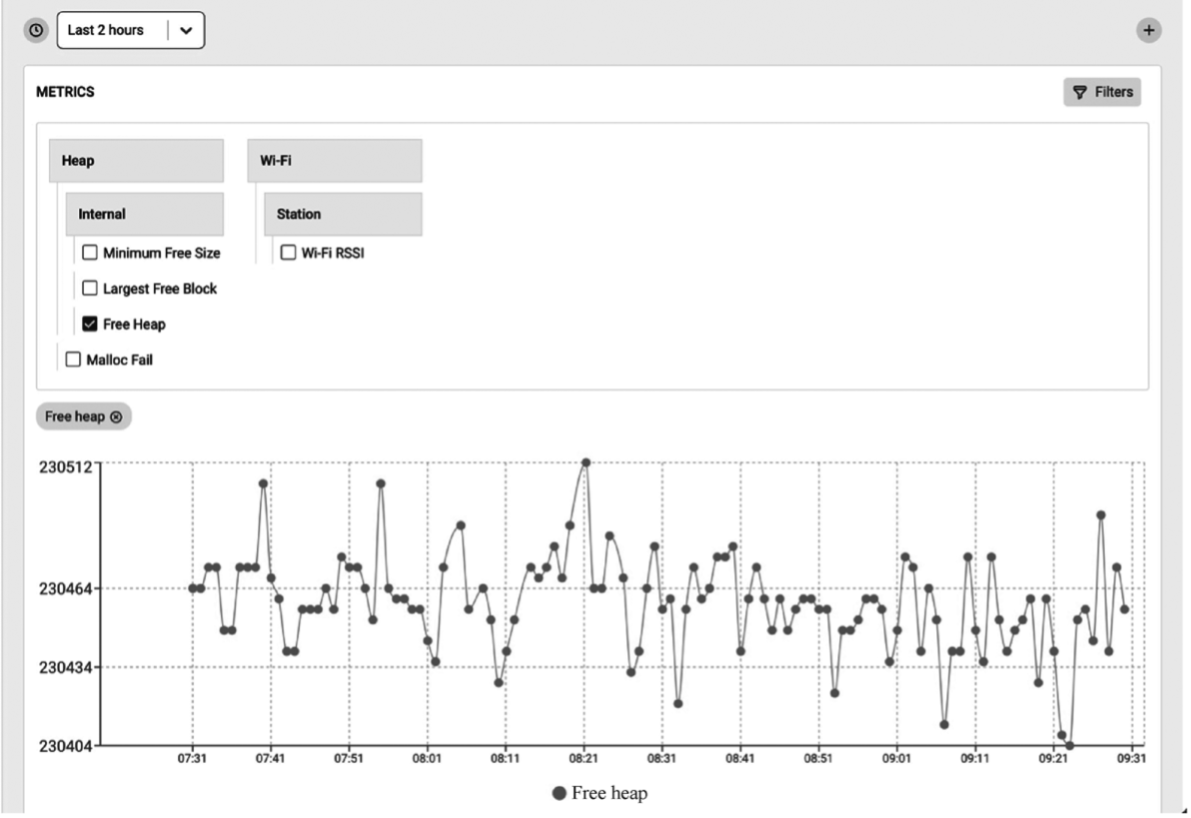
\includegraphics[width=0.85\textwidth]{D15Z/15-5}
    \caption{Metrics information}
\end{figure}

\textbf{1. Heap metrics}

The Insights agent supports reporting free memory, largest free block, and minimum free memory ever. These parameters are tracked and reported for heap in the internal RAM as well as for the heap in the external RAM (in case the device has the PSRAM). The Insights agent also records failed memory allocations, which is available from ESP-IDF v4.2 and onwards.

Set \verb|CONFIG_DIAG_ENABLE_HEAP_METRICS=y| to enable heap metrics.

\textbf{2. Wi-Fi metrics}

The ESP Insights agent also supports Wi-Fi metrics. It collects Wi-Fi signal strength (RSSI), and minimum RSSI information. RSSI is sampled every 30 seconds and if there is a 5 dB difference between the previous count and the current count, it will be reported to the ESP Insights cloud. From ESP-IDF v4.3 onwards, minimum RSSI is also recorded when the RSSI value drops below a pre-configured threshold. The threshold can be configured by calling \verb|esp_wifi_set_rssi_threshold()|. There is also a function which can collect and report Wi-Fi metrics at any given time:

\begin{codebloc}
\begin{tabular}{d}
\verb|1.  /*Reports RSSI to cloud and also prints to console*/|

\verb|2.  esp_diag_wifi_metrics_dump();|
\end{tabular}
\end{codebloc}

\textbf{3. Custom metrics}

Developers can add custom metrics through the following functions.

\begin{codebloc}
\begin{tabular}{d}
\vspace{2pt}
\begin{verbatim}
1.  /*Register a metrics to track room temperature*/
2.  esp_diag_metrics_register("temp", "temp1", "Room temperature", "room",
3.                            ESP_DIAG_ DATA_TYPE_UINT);
4.
5.  /*Record a data point for room temperature*/
6.  uint32_t room_temp = get_room_temperature();
\end{verbatim}
\verb|7.  esp_diag_metrics_add_uint("temp1", &room_temp);|
\end{tabular}
\end{codebloc}

The prototype of the \verb|esp_diag_metrics_register()| function is as follows:

\begin{codebloc}
\begin{tabular}{d}
\vspace{2pt}
\begin{verbatim}
1.  esp_err_t esp_diag_metrics_register(const char *tag, const char *key,
2.                                      const char *label, const char *path,
\end{verbatim}
\verb|3.                                      esp_diag_data_type_t type);|
\end{tabular}
\end{codebloc}

In the prototype of the function \verb|esp_diag_metrics_register()|, the parameter \verb|tag| indicates the label of the metrics, which can be defined by the users. The parameter \verb|key| indicates the unique identifier of the metrics, which is used to find and set the identifier of the metrics. The parameter \verb|label| is the label displayed in the ESP Insights dashboard. The parameter \verb|path| indicates a hierarchical path to the \verb|key|, which must be divided by “.”, e.g \verb|wifi|, \verb|heap.internal|, and \verb|heap.external|. The parameter \verb|type| represents the data type, which supports the following enumeration values:

\begin{codebloc}
\begin{tabular}{d}
\vspace{2pt}
\begin{verbatim}
1.  typedef enum {
2.      ESP_DIAG_DATA_TYPE_BOOL,     /*! < Data type boolean*/
3.      ESP_DIAG_DATA_TYPE_BOOL,     /*! < Data type boolean*/
4.      ESP_DIAG_DATA_TYPE_UINT,     /*! < Data type unsigned integer*/
5.      ESP_DIAG_DATA_TYPE_FLOAT,    /*! < Data type float*/
6.      ESP_DIAG_DATA_TYPE_STR,      /*! < Data type string*/
7.      ESP_DIAG_DATA_TYPE_IPv4,     /*! < Data type IPv4 address*/
8.      ESP_DIAG_DATA_TYPE_MAC,      /*! < Data type MAC address*/
\end{verbatim}
\verb|9.  } esp_diag_data_type_t;|
\end{tabular}
\end{codebloc}

\textbf{4. Variables}

Variables are similar to metrics, but do not need tracing over time since they generally represent information of devices, for example, the IP address of the device. You may set \verb|CONFIG_DIAG_ENABLE_VARIABLES=y| to enable variables support. Like metrics, a set of pre-defined variables are supported, such as IP and Wi-Fi. Additionally, you may add your own custom variables. The variable information is shown in Figure 15.6.

\begin{figure}[!h]
    \centering
    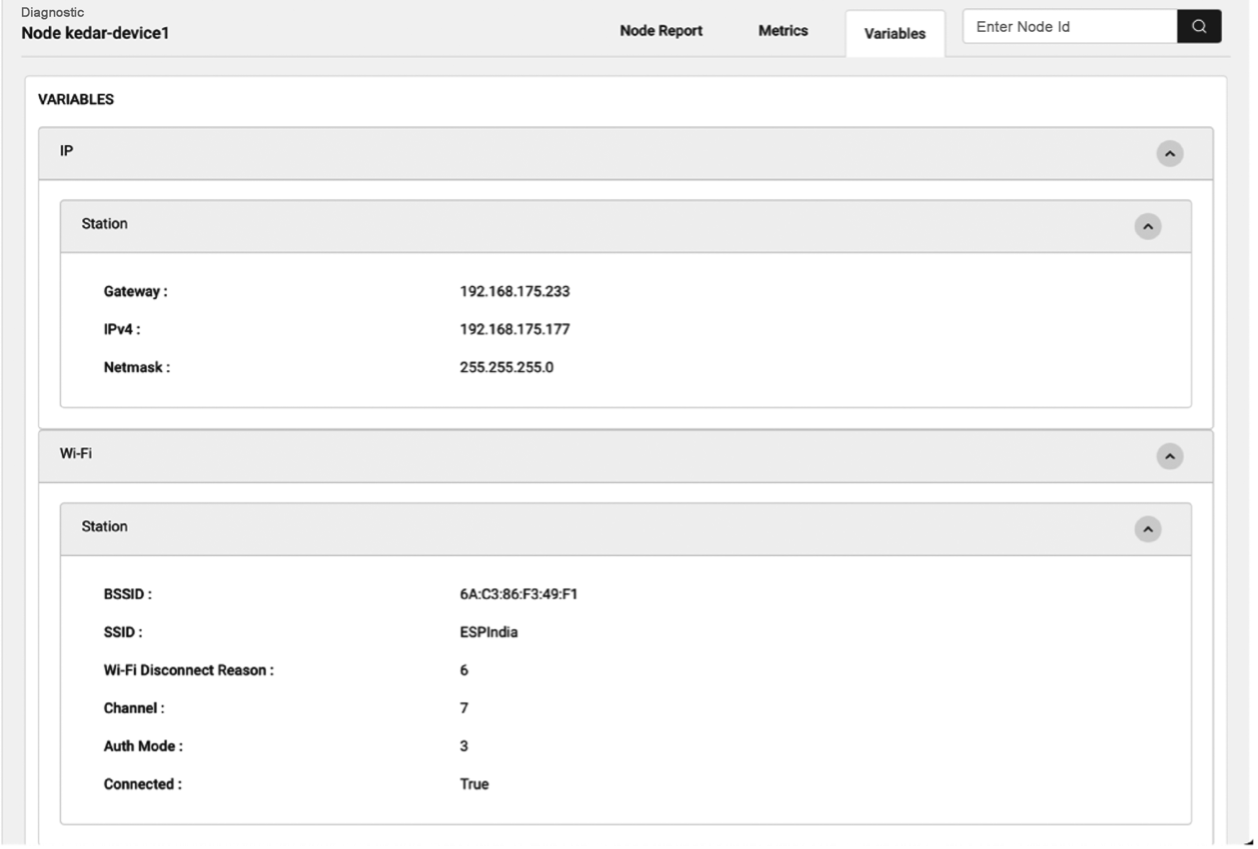
\includegraphics[width=0.8\textwidth]{D15Z/15-6}
    \caption{Variable information}
\end{figure}

\textbf{\textbullet\ Network variables}

As shown in Figure 15.6, ESP Insights currently supports variables in Wi-Fi and IP. For Wi-Fi, supported variables include BSSID, SSID, Wi-Fi disconnection reason, current channel, Wi-Fi connection authentication mode, and connection status. For IP, supported variables include gateway address, IPv4 address, and netmask parameters.

\textbf{\textbullet\ Custom Variables}

Developers can add custom variables through the following functions:

\begin{codebloc}
\begin{tabular}{d}
\vspace{2pt}
\begin{verbatim}
1.  /*Register a variable to track stations associated with ESP32 AP*/
2.  esp_diag_variable_register("wifi", "sta_cnt", "STAs associated",
3.                             "wifi.sta", ESP_DIAG_DATA_TYPE_UINT);
4.
5.  /*Assuming WIFI_EVENT_AP_STACONNECTED and WIFI_EVENT_AP_STADISCONNECTED
6.   events track the number of associated stations*/
\end{verbatim} 
\verb|7.  esp_diag_variable_add_uint("sta_cnt", &sta_cnt);|
\end{tabular}
\end{codebloc}

The prototype of the \verb|esp_diag_metrics_register()| function is as follows:

\begin{codebloc}
\begin{tabular}{d}
\vspace{2pt}
\begin{verbatim}
1.  esp_err_t esp_diag_variable_register(const char *tag, const char *key,
2.                                       const char *label, const char *path,
\end{verbatim} 
\verb|3.                                       esp_diag_data_type_t type);|
\end{tabular}
\end{codebloc}

The parameters of the function \verb|esp_diag_variable_register()| share the same meanings as those of the function \verb|esp_diag_metrics_register()|.

\section{Practice: Using ESP Insights in Smart Light Project}
In Section 15.2, we introduced the use of ESP Insights. In Chapter 9, we introduced how to realise remote control of devices through the ESP RainMaker IoT cloud platform. In this section, we will add ESP Insights to the Smart Light project based on the development in Section 9.4 to realise diagnostics data reporting.

\begin{codebloc}
\begin{tabular}{d}
\vspace{2pt}
\begin{verbatim}
1.  #define APP_INSIGHTS_LOG_TYPE  ESP_DIAG_LOG_TYPE_ERROR 
2.                                  | ESP_DIAG_LOG_TYPE_WARNING 
3.                                  | ESP_DIAG_LOG_TYPE_EVENT
4.  esp_err_t app_insights_enable(void)
5.  {
6.      esp_rmaker_mqtt_config_t mqtt_config = {
7.          .init       		= NULL,
8.          .connect    		= NULL,
9.          .disconnect 		= NULL,
10.         .publish     		= esp_rmaker_mqtt_publish,
11.         .subscribe   		= esp_rmaker_mqtt_subscribe,
12.         .unsubscribe 	= esp_rmaker_mqtt_unsubscribe,
13.     };
\end{verbatim}
\verb|14.     esp_insights_mqtt_setup(mqtt_config);|
\end{tabular}
\end{codebloc}

\begin{codebloc}
\begin{tabular}{d}
\vspace{2pt}
\begin{verbatim}
15.
16.     esp_insights_config_t config = {
17.         .log_type = APP_INSIGHTS_LOG_TYPE,
18.     };
19.     esp_insights_enable(&config);
20.     return ESP_OK;
21. }
22.
23. void app_main()
24. {
25.     ……
26.     /*Enable Schedule*/
27.     esp_rmaker_schedule_enable();
28.
29.     /*Use Insights*/
30.     app_insights_enable();
31.
32.     /*Launch the ESP RainMaker IoT cloud platform server*/
33.     esp_rmaker_start();
34.     ……
\end{verbatim}
\verb|35. }|
\end{tabular}
\end{codebloc}

The code above presents how to use ESP Insights in the ESP-RainMaker example. The \verb|esp_insights_mqtt_setup()| function sets the interface for reporting diagnostics data. In this case, ESP Insights shares the same MQTT channel with the ESP RainMaker IoT cloud platform, which greatly saves the memory. \verb|APP_INSIGHTS_LOG_TYPE| defines the log type that needs to be reported. The current example supports reporting error and warning logs and events. By default, the Insights agent supports uploading device crash logs, so users do not need to configure this type of logs delibrately. Users can enable the following options in the default configuration to record the memory overhead, Wi-Fi signal, and network variables of the device.

\begin{codebloc}
\begin{tabular}{d}
\vspace{2pt}
\begin{verbatim}
1.  CONFIG_DIAG_ENABLE_METRICS=y
2.  CONFIG_DIAG_ENABLE_HEAP_METRICS=y
3.  CONFIG_DIAG_ENABLE_WIFI_METRICS=y
4.  CONFIG_DIAG_ENABLE_VARIABLES=y
\end{verbatim}
\verb|5.  CONFIG_DIAG_ENABLE_NETWORK_VARIABLES=y|
\end{tabular}
\end{codebloc}

In addition, users can customise and report the logs of interest following the introduction in Section 15.2.

\section{Summary}
This chapter introduces ESP Insights, which includes a firmware agent (Insights agent) that runs on the user's device to capture the operating status and abnormality of the device and report them to the ESP Insights cloud. When verifying product functions and on-hook testing, users can log in to the dashboard of the ESP RainMaker IoT cloud platform to view the health status of each device and whether there is an abnormality. Instead of capturing logs of device operation on every device run, logs of device abnormality will be reported to the ESP Insights Cloud. Users can view the reasons for device abnormality clearly through the ESP Insights Cloud interface, making it considerably easier for debugging.

At present, the Insights agent sends data to the ESP RainMaker IoT cloud platform by default. In the future, Espressif will release solutions to support more cloud platforms to receive and process the device information reported by the Insights agent. With these solutions, the functional verification and debugging of the device will become much easier, accelerating the release of user product firmware.

\end{document}